\documentclass[aspectratio=169,11pt]{beamer}

% Frittstående to-siders deck: Mouchel mfl. (2026) vs. Eloundou mfl. (2024).
% Samme preamble som slides/arendalsgata/main.tex slik at rammene kan
% flyttes/\input-es rett inn i arendalsgata- eller FIN-decken.
\usetheme{metropolis}
\metroset{numbering=counter, progressbar=foot}

\usepackage[utf8]{inputenc}
\usepackage[T1]{fontenc}
\usepackage[norsk]{babel}
\usepackage{booktabs}
\usepackage{array}
\usepackage{tikz}
\usepackage{xcolor}
\usepackage{colortbl}
\usepackage{amsmath}
\usepackage{ragged2e}

% Delte stiler fra de andre deckene
% Shared TikZ styles and macros for the exposure-mapping slides.

\usetikzlibrary{positioning, arrows.meta, shapes.geometric, fit, backgrounds, calc}

% Color palette: one color per code system.
\definecolor{cSTYRK}{HTML}{1F4E79}   % STYRK / overlapping ISCO codes: deep blue
\definecolor{cSOC10}{HTML}{C55A11}   % SOC 2010: orange
\definecolor{cSOC18}{HTML}{ED7D31}   % SOC 2018: light orange
\definecolor{cTASK}{HTML}{548235}    % O*NET task: green
\definecolor{cABIL}{HTML}{7030A0}    % O*NET ability: purple
\definecolor{cSCORE}{HTML}{000000}   % final score: black

% A code-system box: \codebox{color}{label}{code}{title}
%   label = "STYRK-08", "SOC 2010", "ISCO-08", ...
%   code  = "2262", "29-1051", ...
%   title = "Pharmacists" / Norwegian name
\tikzset{
  codebox/.style={
    draw=#1, line width=0.6pt,
    rounded corners=2pt,
    inner sep=3pt,
    fill=#1!8,
    text=black,
    align=center,
    minimum width=2.4cm,
    minimum height=0.85cm,
    font=\footnotesize
  },
  taskbox/.style={
    codebox=cTASK,
    minimum width=4cm,
    align=left,
    font=\scriptsize
  },
  chain/.style={
    -{Stealth[length=2mm,width=1.6mm]},
    line width=0.8pt,
    draw=black!50
  },
  arrowlabel/.style={
    font=\scriptsize\itshape,
    text=black!60,
    midway,
    above=2pt,
    fill=white,
    inner sep=1pt
  }
}

% \cbox{color}{label}{code}{title}
\newcommand{\cbox}[4]{%
  \begin{tabular}{c}%
    {\scriptsize\color{#1!85!black}\textbf{#2}}\\[-1pt]%
    {\bfseries #3}\\[-1pt]%
    {\scriptsize #4}%
  \end{tabular}%
}

% Task-table row highlights for Eloundou task scores (requires colortbl).
%   \rR{task}{E}{beta} = score 1.0 row (E_1), light red
%   \rO{task}{E}{beta} = score 0.5 row (E_2), light orange
% Score 0.0 rows are written plain (no cellcolor).
\definecolor{taskRed}{HTML}{FBDADA}
\definecolor{taskOrange}{HTML}{FFE8CC}
\newcommand{\rR}[3]{\cellcolor{taskRed}#1 & \cellcolor{taskRed}#2 & \cellcolor{taskRed}#3}
\newcommand{\rO}[3]{\cellcolor{taskOrange}#1 & \cellcolor{taskOrange}#2 & \cellcolor{taskOrange}#3}

% Palett og TikZ-stiler for illustrasjonsslidene.
% Fargene er hentet fra den private pptx-decken (sam-semesteråpning).
% Hver tekstblokk er en egen node med font=-opsjon, slik at linjeavstanden
% følger fontstørrelsen (fontbytte inne i en node gir feil baselineskip).

\definecolor{illBg}{HTML}{F7F9FC}
\definecolor{illInk}{HTML}{10243E}
\definecolor{illGray}{HTML}{516274}
\definecolor{illPanel}{HTML}{E7EDF4}
\definecolor{illBlue}{HTML}{2F6FB0}
\definecolor{illTeal}{HTML}{2A9D8F}
\definecolor{illOrange}{HTML}{F4A261}
\definecolor{illRed}{HTML}{D65A5A}
\definecolor{illPurple}{HTML}{7566C8}

\newcounter{illnode}

% Kort med farget aksentstripe til venstre:
%   \illcard{(x,y)}{farge}{OVERLINJE}{Tittel}{brødtekst}
% Tegnes inne i en tikzpicture. Kortet er ca. 4.3 cm bredt.
\newcommand{\illcard}[5]{%
  \stepcounter{illnode}%
  \fill[#2] #1 rectangle ($#1+(0.09,-3.6)$);
  \node[anchor=north west, text width=3.9cm, inner sep=0pt,
        font=\scriptsize\bfseries, text=#2]
        (illn\theillnode a) at ($#1+(0.35,-0.05)$) {#3};
  \node[anchor=north west, text width=3.9cm, inner sep=0pt,
        font=\bfseries, text=illInk]
        (illn\theillnode b) at ($(illn\theillnode a.south west)+(0,-0.2)$) {#4};
  \node[anchor=north west, text width=3.9cm, inner sep=0pt,
        font=\scriptsize, text=illGray]
        at ($(illn\theillnode b.south west)+(0,-0.25)$) {#5};
}

% Mørk banner med hvit tekst over hele tekstbredden:
%   \illbanner{tekst}
\newcommand{\illbanner}[1]{%
  \begin{tikzpicture}
    \node[fill=illInk, rounded corners=5pt, text=white, font=\bfseries,
          minimum width=\textwidth, minimum height=0.95cm,
          text width=0.92\textwidth, align=center, inner ysep=6pt] {#1};
  \end{tikzpicture}}

% Trinnkort i prosesskjeden:
%   \illstep{(x,y)}{nr}{Tittel}{spørsmål}         (uten fyll)
%   \illstepx{(x,y)}{nr}{Tittel}{spørsmål}        (uthevet, lys blå plate)
\newcommand{\illstep}[4]{%
  \stepcounter{illnode}%
  \node[anchor=north west, text width=2.6cm, inner sep=0pt,
        font=\small\bfseries, text=illBlue]
        (illn\theillnode a) at ($#1+(0.12,-0.15)$) {#2};
  \node[anchor=north west, text width=2.6cm, inner sep=0pt,
        font=\bfseries, text=illInk]
        (illn\theillnode b) at ($(illn\theillnode a.south west)+(0,-0.18)$) {#3};
  \node[anchor=north west, text width=2.6cm, inner sep=0pt,
        font=\footnotesize, text=illGray]
        at ($(illn\theillnode b.south west)+(0,-0.22)$) {#4};
}
\newcommand{\illstepx}[4]{%
  \fill[illPanel, rounded corners=6pt] ($#1+(-0.18,0.35)$) rectangle ($#1+(2.95,-3.3)$);
  \illstep{#1}{#2}{#3}{#4}%
}
% Pil mellom trinnkort: \illarrow{(x,y)}
\newcommand{\illarrow}[1]{%
  \fill[illGray!70] ($#1+(0,0.09)$) -- ($#1+(0.34,-0.07)$) -- ($#1+(0,-0.23)$) -- cycle;
}

% E-rad for eksponeringskategoriene:
%   \illerow{(x,y)}{farge}{E0}{Skår: 0}{Tittel}{beskrivelse}
\newcommand{\illerow}[6]{%
  \fill[#2] #1 rectangle ($#1+(0.09,-1.55)$);
  \node[anchor=north west, inner sep=0pt, font=\large\bfseries, text=#2]
        at ($#1+(0.35,-0.02)$) {#3};
  \node[anchor=north west, inner sep=0pt, font=\footnotesize\bfseries, text=illGray]
        at ($#1+(1.35,-0.09)$) {#4};
  \node[anchor=north west, inner sep=0pt, font=\bfseries, text=illInk]
        at ($#1+(3.1,-0.05)$) {#5};
  \node[anchor=north west, text width=7.6cm, inner sep=0pt,
        font=\footnotesize, text=illGray]
        at ($#1+(0.35,-0.75)$) {#6};
}


\graphicspath{{./}{../presentation/}{../presentation_no/}{../mapping/}{../../analysis/output/figures/}}

\definecolor{accent}{HTML}{1F4E79}
\setbeamercolor{progress bar}{fg=accent}
\setbeamercolor{title separator}{fg=accent}
\setbeamercolor{frametitle}{bg=accent}
\setbeamercolor{alerted text}{fg=accent}

\begin{document}

% To slides om Mouchel, Bouquet & Sheffi (2026) og forholdet til Eloundou-målet.
% Frittstående kompilering: main.tex i samme mappe. Kan også \input-es i
% arendalsgata- eller FIN-decken (begge laster de samme makroene og har
% analysis/output/figures i \graphicspath).

% ---------------------------------------------------------------
\begin{frame}{To generasjoner av eksponeringsmål}
\begin{columns}[T,onlytextwidth]
\begin{column}{0.475\textwidth}
  {\bfseries\textcolor{illBlue}{Eloundou mfl.\ (2024)}}

  \vspace{0.25em}
  {\footnotesize
  \begin{itemize}\setlength\itemsep{0.25em}
    \item Rubrikk fra GPT-4-æraen: kan en \textbf{språkmodell} halvere tidsbruken? (E0/E1/E2)
    \item Vurdert av mennesker og GPT-4: ekspertenes og modellens \textbf{forhåndsoppfatninger}
    \item Yrkes-$\beta$ = E1 + 0{,}5$\cdot$E2, Core-vektet over O*NET-oppgavene
    \item Øyeblikksbilde av 2023-kapabilitet
  \end{itemize}}
\end{column}
\begin{column}{0.475\textwidth}
  {\bfseries\textcolor{illTeal}{Mouchel mfl.\ (2026)}}

  \vspace{0.25em}
  {\footnotesize
  \begin{itemize}\setlength\itemsep{0.25em}
    \item Rubrikk for \textbf{agentisk KI 2026}: verktøy- og nettleserbruk gir direkte eksponering; ny E3-klasse for syn
    \item \textbf{Evidensbasert}: oppgavene vurderes mot 30\,000 nyhetsartikler og 24\,000 forskningssammendrag
    \item Ensemble av sju åpne modeller; oppgavetids-vekting til yrkes-skår
    \item To armer: \textbf{A1} (teoretisk) og S0 (kalibrert mot faktisk Claude-bruk)
  \end{itemize}}
\end{column}
\end{columns}

\vspace{0.25em}
\illbanner{Samme oppgave-for-oppgave-$\beta$, men med 2026-kapabilitet og dokumentert evidens.}

\vspace{0.05em}
\raggedright\tiny\textcolor{illGray}{Kilder: Eloundou mfl.\ (Science, 2024); Mouchel, Bouquet \& Sheffi (2026), arXiv:2605.15474 (dataversjon 2026-07-20).}
\end{frame}

% ---------------------------------------------------------------
\begin{frame}{Nytt mål, nesten samme rangering av yrker}
\begin{columns}[T,onlytextwidth]
\begin{column}{0.54\textwidth}
  \centering
  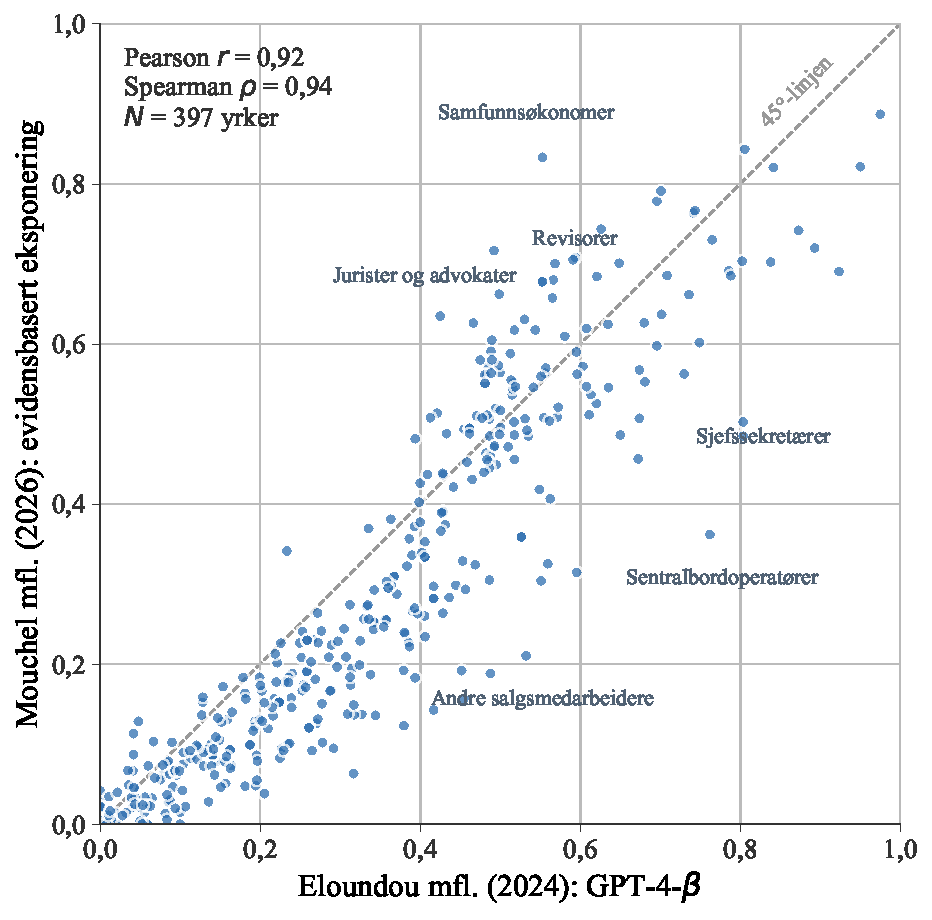
\includegraphics[height=0.8\textheight]{figure_mouchel_vs_eloundou.pdf}
\end{column}
\begin{column}{0.44\textwidth}
  \vspace{0.3em}
  {\footnotesize
  \begin{itemize}\setlength\itemsep{0.35em}
    \item Ett punkt per yrke (397 STYRK-08-koder), samme SOC--ISCO-krysskobling
    \item Korrelasjon \textbf{0{,}92} (Pearson), \textbf{0{,}94} (Spearman); 66 prosent i samme femtedel, 99 prosent innen én
    \item \textcolor{illTeal}{\textbf{Opp}} med agentisk rubrikk: jus, samfunnsøkonomi, revisjon, rådgivning
    \item \textcolor{illRed}{\textbf{Ned}}: sentralbord, sekretær- og annet rutinearbeid, der evidensen viser mindre reell tidsbesparelse
  \end{itemize}}

  \vspace{0.35em}
  {\footnotesize\bfseries\textcolor{illInk}{Resultater bygget på Eloundou-femdelene står seg med 2026-målet.}}
\end{column}
\end{columns}

\vspace{0.05em}
\raggedright\tiny\textcolor{illGray}{Kilde: egne beregninger. Mouchel = A1-armen (ukalibrert, uavhengig av Claude-bruksdata); Eloundou = GPT-4-$\beta$ fra kiindeksen.}
\end{frame}


\end{document}
